\section{Innere Produkte}
In diesem Kapitel sei stets $\mathbb{K}=\mathbb{R}$ oder $\mathbb{K}=\mathbb{C}$.  Wir beschränken uns weiter auf reelle oder komplexe lineare Räume $X$.  Insbesondere im Fall $\K = \Co$ erinnern wir an das komplex-konjugierte
\[\overline{z}=(x,-y)=x-iy\]
einer komplexen Zahl $z=(x,y)=x+iy$, sowie ihren Betrag $\left|z\right|:=\sqrt{zz}=\sqrt{x^2+y^2}$.  Wir betrachten $\R$ als Teilmenge von $\Co$ und erhalten: $z=\overline{z}\Leftrightarrow z\in \R$.
\subsection{Skalarprodukte und Orthogonalität}
\subsubsection{Definition (inneres Produkt)}
Ein \underline{inneres Produkt} auf $X$ ist eine Abbildung $\langle\cdot ,\cdot \rangle\colon X\times X\rightarrow \K$ mit
\romannum
\begin{enumerate}
\item $\langle\alpha x+\beta y,z\rangle=\alpha \langle x,z\rangle+\beta \langle y,z\rangle$ (\underline{Linearität im 1. Argument})
\item $\langle x,y\rangle=\overline{\langle y,x\rangle}$ (\underline{konjugierte Symmetrie})
\item $\langle x,x\rangle\geq 0$ und Gleichheit genau für $x=0$ (\underline{positive Definitheit})
\end{enumerate}
Für alle $x,y,z\in X,\ \alpha,\beta \in \K$.  Ein linearer Raum mit innerem Produkt heißt auch \underline{Prä-Hilbert-Raum}.\\
Statt innerem Produkt sagt man auch \underline{Skalarprodukt}.
\subsubsection{Bemerkung}
\numbers
\begin{enumerate}
\item Aufgrund der konjugierten Symmetrie ist stets $\langle x,x\rangle\in \R$, während die positive Definitheit $\langle x,x\rangle>0$ für $x\not=0$ garantiert.
\item Ein inneres Produkt ist \underline{Semilinear} im 2. Argument:
\[\phantomsection\label{5.1a}(5.1a)\ \langle x,\alpha y+\beta z\rangle=\overline{\alpha }\langle x,y\rangle+\overline{\beta }\langle x,z\rangle\text{ für alle } x,y,z \in X,\ \alpha, \beta \in \K\]
\item Unter einer \underline{Norm} auf $X$ versteht man die Funktion
\[\|\cdot \|\colon X\rightarrow \R,\ \|x\| :=\sqrt{\langle x,x\rangle}\]
Insbesondere gilt $\|x\|=0\Leftrightarrow x=0$.  Zu jedem $x\not=0$ nennen wir $y:=\frac{1}{\|x\|}x$ den \underline{normierten Vektor} zu $x$, denn $\|y\|=1$.
\end{enumerate}
\subsubsection{Bemerkung (Orthogonalität)}
\begin{enumerate}
\item Die Elemente $x,y\in X$ heißen \underline{orthogonal}, falls $\langle x,y\rangle=0$.  Die resultierende Relation 
\[x \bot y :\Leftrightarrow \langle x,y\rangle=0\]
ist symmetrisch aber nicht transitiv.  Wegen $\langle x,0\rangle=\langle0,x\rangle=0$ ist $0\in X$ orthogonal zu jedem $x\in X$.
\item Die Teilmengen $Y_1,Y_2\subseteq X$ heißen \underline{orthogonal}, insofern
\[\langle y_1,y_2\rangle=0\text{ für alle }y_1\in Y_1,\ y_2\in Y_2\]
\end{enumerate}
\subsubsection{Beispiel (Euklidischer Raum)}
$\R ^n$ mit $\langle x,y\rangle:=\sum _{j=1}^n x_jy_,$, $\|x\|=\sqrt{\sum _{j=1}^nx_j^2}$
\subsubsection{Beispiel (Unitärer Raum)}
$\Co ^n$ mit $\langle x,y\rangle=\sum _{j=1}^n x_j \overline{y_j}$, $n=1$, $\langle i,i\rangle=i\cdot (-1)=1$.
\subsubsection{Beispiel}
\label{5.1.6}
\numbers
\begin{enumerate}
\item Mit sogenannten Gewichten $\omega_1,\dots,\omega_n>0$ ist auch $\langle x,y \rangle_\omega=\sum_{j=1}^n \omega_j x_j \overline{y}_j$ ein inneres Produkt auf $\K^n$ mit induzierter Norm $\|x\|_\omega= \sqrt{\sum_{j=1}^n \omega_j |x_j|^2}$
\item Mit einer stetigen Gewichtsfunktion $\omega:[a,b]\rightarrow(0,\infty)$, $a<b$ sind auch die stetigen Funktionen $X=C([a,b],\K)$ ein linearer Raum mit innerem Produkt
\[\phantomsection\label{5.1b}(5.1b)\ \langle x, y\rangle_\omega:=\int_a^b \omega(t)x(t)\overline{y(t)}dt\]
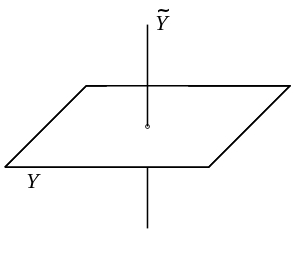
\includegraphics[scale=0.4]{5-1-6.jpg}
\end{enumerate}
\subsubsection{Definition (Orhtogonales Komplement)}
Es sei $S \subseteq X$. Dann heißt $S^\bot:=\{x\in X:\langle x,y \rangle =0\text{ für alle }y\in S\}$
 das \underline{orthogonale Komplement} von $S$ (in X)
\subsubsection{Beispiel}
\numbers
\begin{enumerate}
\item Es ist $\{0\}^\bot=X$ und $X^{\bot}=\{0\}$
\item Im Raum $X=\R^3$ haben wir in \hyperref[2.5.2]{Beispiel \ref*{2.5.2}} nachgewiesen, dass die Gerade $\tilde{Y}:=\R\begin{pmatrix}1 \\1 \\1\end{pmatrix}$ ein Komplement zur Ebene $Y:=\{x\in X, x_1-x_2+x_3=0\}=\R\begin{pmatrix}1\\1\\0\end{pmatrix}+\R\begin{pmatrix}1\\0\\-1\end{pmatrix}$ ist.
Betrachtet man $\R^3$ als Euklidischen Raum, so ist $\tilde{Y}$ wegen $\left\langle \begin{pmatrix}1 \\1 \\1\end{pmatrix},\begin{pmatrix}1 \\1 \\0\end{pmatrix}\right\rangle=2$ jedoch kein orthogonales Komplement von Y, vielmehr gilt $Y^{\bot}=\R\begin{pmatrix}1 \\-1 \\1\end{pmatrix}$
\end{enumerate}
\subsubsection{Proposition}
\label{5.1.9}
Für jedes $S\subseteq X$ ist $S^{\bot}$ ein Unterraum von $X$ mit $(span\ S)\cap S^{\bot}=\{0\}$.\\
\underline{Beweis}: Es seien $x_1,x_2\in S^{\bot}$ und wir erhalten $\langle \alpha_1 x_1+\alpha_2 x_2,y\rangle=\alpha_1\langle x_1,y\rangle+\alpha_2\langle x_2,y\rangle=0$ für alle $\alpha_1,\alpha_2\in\K$ $y\in S$ dies garantiert $\alpha_1 x_1+\alpha_2 x_2\in S^{\bot}$ und $S^{\bot}$ ist ein linearer Raum.
Weiter sei $x\in\ S^{\bot}$ und $x\in span~S$, d.h. $x=\sum_{i=1}^n \xi_i x_i$ mit Koeffizienten $\xi_i\in \K$ und $x_i\in S$. Dies impliziert $\langle x,x\rangle=\langle \sum_{i=1}^n \xi_i x_i,x\rangle=\sum_{i=1}^n\xi_i \underbrace{\langle x_i,x\rangle}_{=0\text{ weil }x\in S^{\bot}}=0$ und folglich $x=0$.
\subsubsection{Satz}
Ist $dimX<\infty$ und $Y$ ein Unterraum von $X$, so gilt
\alphabet
\begin{enumerate}
\item $X=Y\oplus Y^{\bot}$
\item $(Y^{\bot})^{\bot}=Y$
\item $dimX=dimY+dimY^{\bot}$
\end{enumerate}
\underline{Beweis (a)}: $Y\cap Y^{\bot}=\{0\}$ gilt nach \hyperref[5.1.9]{Proposition \ref*{5.1.9}}. Es bleibt $X=Y\oplus Y^{\bot}$ zu zeigen. Zu jedem $x\in X$ muss es also $y\in Y$ und $y^{\bot}\in Y^{\bot}$ mit $x=y+y^{\bot}$ geben. Ist $\{y_1, \dots,y_n\}$ eine Orthonormalbasis von $Y$, so definieren wir
\[y:=\sum_{i=1}^m \langle x,y_i\rangle \cdot y_i,\qquad y^{\bot}:=x-y\text{ usw.}\]
\subsubsection{Definition (Orthogonal- und Orthonormalbasis)}
Eine Familie $\mathcal{S} \subseteq X$ heißt
\alphabet
\begin{enumerate}
\item \underline{orthogonal}, falls $\langle x,y\rangle=0$, für alle $x,y\in \mathcal{S}$ $x\neq y$
\item \underline{orthonormal}, falls $\langle x,y\rangle=\begin{cases}1,x=y\\0,x\neq y\end{cases}$, für $x,y\in \mathcal{S}$
\end{enumerate}
Eine Orthogonal- bzw. Orthonormalbasis von X ist eine orthogonale bzw. orthonormale Basis von X.\\
Jede orthonormale Familie ist auch orthogonal.
\subsubsection{Beispiel}
\numbers
\begin{enumerate}
\item Die Standardbasis $\epsilon_n=\{e_1,\dots,e_n\}$ aus \hyperref[standardbasis]{Beispiel \ref*{standardbasis}} ist eine Orthonormalbasis des Euklidischen Raums $\R^n$ wie auch des unitären Raums $\Co^n$.
\item Die Legendre Polynome $p_n\in P(\R)$, $p_n(t)=\frac{1}{2^n n!} \frac{d^n}{dt^n} (t^2-1)^n$ für $n\in\N_0$ definieren eine orthogonale Familie $\{p_n\}_{n\in\N_0}$ bzgl. dem inneren Produkt (\hyperref[5.1b]{$5.1b$}) aus \hyperref[5.1.6]{Beispiel \ref{5.1.6}(2)} mit $\omega(t)=1$ auf $[-1,1]$
\item Wir definieren die trigonometrischen Funktionen $c_n,s_n:[-\pi,\pi]\rightarrow\R$, $c_n(t):=cos(nt)$, $s(t):=sin(nt)$ mit $n\in\N_0$. Dann ist $\mathcal{S}:=\{c_n\}_{n\in\N_0} \cup \{s_n\}_{n\in\N}$ eine orthogonale Familie in $C([-\pi,\pi],\R)$ bezüglich (\hyperref[5.1b]{$5.1b$}) mit $\omega(t)=1$ auf $[-\pi,\pi]$.
\end{enumerate}
\subsubsection{Proposition}
Jede orthogonle Familie $\mathcal{S}\subseteq X$ mit $0\notin\mathcal{S}$ ist linear unabhängig.\\
\underline{Beweis}: Es sei $\{x_1,\dots,x_n\}$ eine endliche Teilfamilie von $\mathcal{S}$ und $\sum_{j=1}^n \xi_j x_j =0$ mit Koeffizienten $\xi_j\in\K$.
Dann resultiert $0=\langle 0,x_k\rangle=\langle\sum_{j=1}^n\xi_j x_j,x_k\rangle=\sum_{j=1}^n \xi_j \langle x_j,x_k\rangle=\xi_k\langle x_j,x_k\rangle$ für alle $1\leq k\leq n$. Wegen $x_k\neq 0$ folgt $\xi_k=0$.\\
Vorteil von Orthonormalbasen: Koordinaten einfach berechenbar
\subsubsection{Proposition}
Ist $\{x_1,\dots,x_n\}$ eine Orthonormalbasis von $X$ so gilt $x=\sum_{j=1}^n \langle x,x_j\rangle x_j$ für alle $x\in X$.\\
\underline{Beweis}: Da $\{x_1,\dots,x_n\}$ orthonormal ist, gilt $\langle x_j,x_k\rangle=\delta_{jk}$ für $1\leq j,k\leq n$. Die Koeffizienten $\xi_j\in\K$ eines beliebigen $x=\sum_{j=1}^n\xi_j x_j \qquad \xi_k=\sum_{j=1}^n\xi_k \underbrace{\langle x_j,x_k\rangle}_{\delta_{jk}}=\langle\sum_{j=1}^n\xi_j x_j,x_k\rangle=\langle x,x_k\rangle$\\
Berechnung von Orthogonal- bzw. Orthonormalbasis aus einer gegebenen Basis: Orthogonalisierungsverfahren von Gram-Schmidt:

\numbers
\begin{enumerate}
\setcounter{enumi}{-1}
\item Es sei eine linear unabhängige Familie $\mathcal{S}=\{x_1,x_2,x_3,\dots\}$ gegeben auf $X$ mit innerem Produkt $\langle \cdot,\cdot\rangle$
\item Setze $y_1=x_1$
\end{enumerate}
